% THE PYTHAGOREAN THEOREM - WORKSHEET 0 (IN-CLASS INSTRUCTION)
\documentclass[12pt, letterpaper, fleqn]{article}

% ----------------------------------------------------------
% PACKAGES
% ----------------------------------------------------------
\usepackage{graphicx}
\usepackage{xcolor}
\usepackage[most]{tcolorbox}
\usepackage{amsmath, amssymb}
\usepackage{fancyhdr}
\usepackage[utf8]{inputenc}
\usepackage[T1]{fontenc}
\usepackage{enumitem}
\usepackage{geometry}
\usepackage{tikz}
\usepackage{needspace}
\usepackage{multicol}

\usetikzlibrary{arrows.meta, calc, positioning}

% ----------------------------------------------------------
% PAGE SETUP
% ----------------------------------------------------------
\usepackage{times}
\geometry{letterpaper, top=1.25in, bottom=1.25in, marginpar=0.5in}

% ----------------------------------------------------------
% HEADER / FOOTER
% ----------------------------------------------------------
\newcommand{\logowidth}{3cm}
\setlength{\headheight}{20pt}
\setlength{\footskip}{40pt}

\pagestyle{fancy}
\fancyhf{}
\fancyhead[C]{\small\bfseries The Pythagorean Theorem}
\fancyfoot[L]{\raisebox{2pt}{
\includegraphics[width=\logowidth]{../kss.png}}}
\fancyfoot[C]{\thepage}
\fancyfoot[R]{8.22.0}

\renewcommand{\footrulewidth}{0.2pt}

% ----------------------------------------------------------
% THEME COLOR
% ----------------------------------------------------------
\definecolor{customteal}{HTML}{2fbdb9}

% ----------------------------------------------------------
% HELPER MACROS
% ----------------------------------------------------------
\newcommand{\blank}{\underline{\hspace{2.2cm}}}
\newcommand{\blanklong}{\underline{\hspace{6.5cm}}}
\newcommand{\blankshorter}{\underline{\hspace{1.5cm}}}

% ----------------------------------------------------------
% DOCUMENT
% ----------------------------------------------------------
\begin{document}

\textbf{Name:} \underline{\hspace{5cm}}
\hfill
\textbf{Date:} \underline{\hspace{3cm}}\\

% ==========================================================
% SECTION 1: FOUNDATION
% ==========================================================
\begin{tcolorbox}[colback=customteal!20]
    \large\textcolor{black}{\textbf{Foundation: Right Triangles and the Formula}}
\end{tcolorbox}

\vspace{3mm}

\noindent
The \textbf{Pythagorean Theorem} is a special rule that only applies to \textbf{right triangles} (triangles with one $90^\circ$ angle). It describes the relationship between the three sides.

\begin{itemize}
    \item \textbf{Legs ($a$ and $b$):} The two shorter sides that form the right angle.
    \item \textbf{Hypotenuse ($c$):} The longest side of the triangle. It is always directly across from the right angle.
    \item \textbf{The Formula:} $a^2 + b^2 = c^2$. If you square the two legs and add them together, it equals the square of the hypotenuse.
\end{itemize}

\vspace{4mm}

% ==========================================================
% VISUAL REPRESENTATION
% ==========================================================
\begin{tcolorbox}[colback=white, colframe=black!25, boxrule=0.6pt, arc=4mm, left=6mm, right=6mm, top=5mm, bottom=5mm]

\textbf{Visual Representation: The 3-4-5 Triangle}

\medskip

\begin{center}
\begin{tikzpicture}[scale=0.8]

% Triangle
\draw[thick, blue] (0,0) -- (4,0) node[midway, below] {$a=4$};
\draw[thick, red] (0,0) -- (0,3) node[midway, left] {$b=3$};
\draw[thick, green!60!black] (4,0) -- (0,3) node[midway, above right] {$c=5$};

% Right angle marker
\draw (0.3, 0) -- (0.3, 0.3) -- (0, 0.3);

% Squares
\draw[dashed, blue] (0,0) rectangle (4,-4);
\node[blue] at (2,-2) {$a^2 = 16$};

\draw[dashed, red] (0,0) rectangle (-3,3);
\node[red] at (-1.5,1.5) {$b^2 = 9$};

% Hypotenuse Square
\begin{scope}[shift={(4,0)}, rotate=143.13]
    \draw[dashed, green!60!black] (0,0) rectangle (5,5);
    \node[green!60!black, rotate=-143.13] at (2.5, 2.5) {$c^2 = 25$};
\end{scope}

\end{tikzpicture}
\end{center}

\medskip
Notice that $16 + 9 = 25$. The area of the squares on the two legs adds up to the area of the square on the hypotenuse!

\end{tcolorbox}

\vspace{4mm}

\newpage

% ==========================================================
% WORKED EXAMPLES
% ==========================================================
\begin{tcolorbox}[colback=customteal!20]
\large\textcolor{black}{\textbf{Finding Missing Sides}}
\end{tcolorbox}

\noindent
We can use the formula to find a missing hypotenuse, or a missing leg. Remember to take the square root as your final step!

\vspace{3mm}

\begin{tcolorbox}[colback=white, colframe=black!25, boxrule=0.6pt, arc=4mm, left=6mm, right=6mm, top=5mm, bottom=5mm]

\textbf{Worked Example 1: Finding a Missing Leg}

\medskip

\textbf{Problem:} A right triangle has a hypotenuse of $13\text{ cm}$ and one leg of $5\text{ cm}$. Find the length of the other leg.

\medskip

\textbf{Solution:}
\begin{itemize}
    \item \textbf{Step 1 (Identify a, b, c):} $c = 13$, $a = 5$, $b = ?$ (it doesn't matter which leg is a or b).
    \item \textbf{Step 2 (Plug into formula):} $5^2 + b^2 = 13^2$
    \item \textbf{Step 3 (Square the numbers):} $25 + b^2 = 169$
    \item \textbf{Step 4 (Solve for $b^2$):} Subtract $25$ from both sides.
    \[ b^2 = 144 \]
    \item \textbf{Step 5 (Square root):} Take the square root of both sides to get just $b$.
    \[ b = \sqrt{144} = 12 \]
    \item The missing leg is $12\text{ cm}$.
\end{itemize}

\end{tcolorbox}

\vspace{4mm}

% ==========================================================
% PRACTICE 1
% ==========================================================
\begin{tcolorbox}[colback=white!15, colframe=black, boxrule=1.5pt, arc=4mm, left=6mm, right=6mm, top=5mm, bottom=5mm]

\textbf{Guided Practice: Basic Operations}

\medskip

\noindent
\textbf{1.} Find the hypotenuse if the legs are $6$ and $8$.
\vspace{2cm}

\noindent
\textbf{2.} Find the missing leg if the hypotenuse is $10$ and one leg is $8$.
\vspace{2cm}

\noindent
\textbf{3.} Do the side lengths $5, 12, \text{ and } 14$ form a right triangle? (Hint: Does $a^2 + b^2 = c^2$?)
\vspace{2cm}

\end{tcolorbox}

\newpage

% ==========================================================
% THINKING PROBLEM
% ==========================================================
\begin{tcolorbox}[colback=customteal!20]
\large\textcolor{black}{\textbf{Deeper Thinking: Real-World Applications}}
\end{tcolorbox}

\vspace{3mm}

\begin{tcolorbox}[colback=white!15, colframe=black, boxrule=1.5pt, arc=4mm, left=6mm, right=6mm, top=5mm, bottom=5mm]

\textbf{Deeper Thinking Problem 1: The Leaning Ladder}

\medskip

\noindent
A $15\text{-foot}$ ladder is leaning against a vertical brick wall. The base of the ladder is exactly $9\text{ feet}$ away from the bottom of the wall. 

\vspace{5mm}

\noindent
\textbf{a)} Draw a diagram of this situation. Label the ladder, the wall, and the ground. Which of these represents the hypotenuse?

\vspace{4cm}

\noindent
\textbf{b)} Use the Pythagorean theorem to find how high up the wall the ladder reaches.

\vspace{4cm}

\noindent
\textbf{c)} If you move the base of the ladder so it is only $5\text{ feet}$ away from the wall, will the top of the ladder go higher or lower? (You don't need to calculate the exact number, just explain the logic).

\vspace{2.5cm}

\end{tcolorbox}

\end{document}
\end{document}
